\documentclass{article}
\newcommand\tab[1][1cm]{\hspace*{#1}}
\usepackage[utf8]{inputenc}
\usepackage{rotating}

\title{CSE211 Homework1}
\author{Yakup Talha Yolcu }


\begin{document}

\maketitle

\section{Problem 1}
\begin{itemize}
    \item a) If it snows tonight, then I will stay at home.
    \newline
    Converse:If I will stay at home, it snows tonight.
    
    Contrapositive:If I will not stay at home, it doesn't snow tonight
    
    Inverse:If it doesn't snow tonight, I will not stay at home
    \newline
    
    \item b) I go to the beach whenever it is a sunny summer day.
    
    Converse: It is a sunny summer day whenever I go to the beach
    
    Contrapositive:Neither it is not a sunny summer day nor I go to the beach 
    
    Inverse:I don't go to the beach and It is not a sunny summer day
    \newline
    
    \item c)If I stay up late, then I sleep until noon
    
    Converse:If I sleep until noon then I stay up late
    
    Contrapositive:If I don't sleep until noon then I don't stay up late
    
    Inverse:If I don't stay up late then I don't sleep until noon
    
 
\section{Problem 2}
    \item a) (p $\bigoplus$ $\rightharpoondown$ q)
    \begin{table}[]
    \begin{tabular}{|l|l|l|l|}
    \hline
    p & q & $\rightharpoondown$ q & p $\bigoplus$ $\rightharpoondown$q \\ \hline
    T & T & F   & T              \\ \hline
    T & F & T   & F              \\ \hline
    F & T & F   & F              \\ \hline
    F & F & T   & T              \\ \hline
    \end{tabular}
    \end{table}
   \newline
   \newline\newline
  
\item (b) (p $\Leftrightarrow$ q) $\bigoplus$ (¬ p $\Leftrightarrow$ ¬ r)
\end{itemize}

\begin{itemize}

\begin{table2}[]
\begin{tabular}{|l|l|l|l|l|l|l|}
\hline
p & q & r & $$\rightharpoondown$$ r & p $\Leftrightarrow$ q & $\rightharpoondown$ p $\Leftrightarrow$ $\rightharpoondown$ r & (p $\Leftrightarrow$ q) $\bigoplus$ ( $\rightharpoondown$ p $\Leftrightarrow$ $\rightharpoondown$ r) \\ \hline
T & T & T & F  & T                   & F                           & T                                                             \\ \hline
T & T & F & T  & T                   & T                           & F                                                             \\ \hline
T & F & F & T  & F                   & T                           & T                                                             \\ \hline
T & F & T & F  & F                   & F                           & F                                                             \\ \hline
F & T & T & F  & F                   & T                           & T                                                             \\ \hline
F & T & F & T  & F                   & F                           & F                                                             \\ \hline
F & F & F & T  & T                   & F                           & T                                                             \\ \hline
F & F & T & F  & T                   & T                           & F                                                             \\ \hline
\end{tabular}
\end{table2}
\end{itemize}

\begin{itemize}
 \item (c) (p  $\bigoplus$ q) $\Rightarrow$ (p $\bigoplus$ $\rightharpoondown$ q)  
\end{itemize}



 \begin{table3}[]
\begin{tabular}{|l|l|l|l|l|l|}
\hline
p & q & $\rightharpoondown$q & p $\bigoplus$ q & p $\bigoplus$ $\rightharpoondown$ q & \begin{tabular}[c]{@{}l@{}}(p  $\bigoplus$q) $\Rightarrow$ (p  $\bigoplus$  $\rightharpoondown$ q)
\end{tabular} \\ \hline
T & T & F                    & F               & T                                   & T                                                                                                                   \\ \hline
T & F & T                    & T               & F                                   & F                                                                                                                   \\ \hline
F & T & F                    & T               & F                                   & F                                                                                                                   \\ \hline
F & F & T                    & F               & T                                   & T                                                                                                                   \\ \hline
\end{tabular}
\end{table3}

\section{Problem 3}

\begin{itemize}
    \item P(x): ”x can speak English.”
    \item Q(x): ”x knows Python.”
    \item H(x): ”x is happy.”
\end{itemize}    
    
    (a) There is a student at the university who can speak English and who knows Python.\newline
    (Solution)
    \exists x (P(x) \wedge Q(x)) \newline
    
    (b) There is a student at the university who can speak English but who doesn’t know Python. \newline
    (Solution)
    \exists x (P(x) \wedge $\rightharpoondown$ Q(x)) \newline
    
    (c) Every student at the university either can speak English or knows Python.\newline
    (Solution)
    \forall x (P(x) \vee Q(x)) \newline
    
    (d) No student at the university can speak English or knows Python.\newline
    (Solution)
    \exists x(P(x) \vee Q(x)) \newline
    
    (e) If there is a student at the university who can speak English and know Python, then she/he is happy.\newline
    (Solution)
    \exists x((P(x) \wedge Q(x)) \Rightarrow H(x)) \newline
    
    (f ) At least two students are happy. \newline
    (Solution)
    \exists  x1  \exists  x2 (P(x1),P(x2)) \newline
    
    (g) $\neg \forall x (Q(x) \wedge P(x))$ \newline
    (Solution) "There is not a student who knows Python and there is not a student can speak English"
    
    
    \section{Problem 4}
    
    Prove that 3 + 3 . 5 + 3 . $5^2$ + . . . + 3 . $5^n$ =$\frac{3(5^{n+1} - 1)}{4}$ whenever n is a nonnegative integer.\newline
    Solution:
    
    In Mathematical Induction we try for n=1 \newline
    1st step:For n=1 Equation becomes:
   3 + 3.5=$\frac{3(5^{1+1} - 1)}{4}$ so 18=18 n=1 satisfies this equation\newline
   
   2nd step:We accept that equation satisfies for n=k \newline
   3 + 3 . 5 + 3 . $5^2$ + . . . + 3 . $5^k$ =$\frac{3(5^{k+1} - 1)}{4}$\newline
   
   3rd step:We will try for n=k+1 to prove the equation\newline \newline
   3 + 3 . 5 + 3 . $5^2$ + . . . + 3 . $5^k$ + 3 . $5^{k+1}$ =$\frac{3(5^{k+1+1} - 1)}{4}$
   \newline \newline
   If we subtitue 2nd step equation from 3rd step equation we will get:\newline\newline
   3 . $5^{k+1}$=$\frac{3(5^{k+1+1} - 1)}{4}$ - $\frac{3(5^{k+1} - 1)}{4}$  If we multiply by 4 and divide by 3 two side of the equation we will get:\newline\newline
   4 . $5^{k+1}$ = ($5^{k+2}$ -1) - ($5^{k+1}$ -1) \newline
   20 . $5^{k}$ = $5^{k}$ . 25 - 1 - $5^{k}$ . 5 + 1\newline
   20 . $5^{k}$ = 20 . $5^{k}$ \newline
   So for n=k+1 equation is satisfied and it means that this equation is true\newline
   
   \section{Problem 5}
   Prove that $n^2$ - 1 is divisible by 8 whenever n is an odd positive integer \newline
   Solution:
   
   Let's say n=2k-1 because of the term that n is an odd positive integer \newline
   For Inductıon's 1st step, let's say n=3\newline
   3$^2$-1 $\equiv$ 0 (mod 8)\newline
   8 $\equiv$ 0 (mod 8)\newline
   \newline
   For Induction's 2st step accept this equation satisfies for n=2 . k - 1\newline
   (2 . k - 1) $^2$ - 1 $\equiv$ 0 (mod 8)\newline
   4 . k $^2$ - 4 . k + 1 - 1 $\equiv$ 0 (mod 8) \newline
   4 . k $^2$ - 4 . k $\equiv$ 0 (mod 8) \newline
   
   For Induction's 3rd step, we will try for n = 2 . k  + 1 (n is still odd positive integer) \newline
   (2 .k + 1) $^2$ - 1 $\equiv$ 0 (mod 8)\newline
   4 .k $^2$ + 4 .k + 1 - 1 $\equiv$ 0 (mod 8) we can write 4 .k $^2$ + 4.k as 4 .k $^2$ - 4 .k + 8.k \newline
   4 . k $^2$ - 4 . k + 8 . k $\equiv$ 0 (mod 8) $\tab$ 4 . k $^2$ - 4 . k was divisible by 8  \newline
   8 . k $\equiv$ 0 (mod 8) this equation satisfies the main equation\newline
   We concluded that $n^2$ - 1 is divisible by 8 whenever n is an odd positive integer \newline
   
   
   
   \section{Problem 6}
   
   Which of the following sets are equal? Show your work step by step.\newline
a) $\{$t : t is a root of $x^2$ – 6x + 8 = 0$\}$
\newline
b) $\{$y : y is a real number in the closed interval [2, 3]$\}$
\newline
c) $\{$4, 2, 5, 4$\}$
\newline
d) $\{$4, 5, 7, 2$\}$ - $\{$5, 7$\}$
\newline
e) $\{$q: q is either the number of sides of a rectangle or the number of digits in any integer between 11 and 99$\}$\\ \newline

Solution:
a)roots of the $x^2$ – 6x + 8 = 0$\}$ can be find by factoring\newline
(x-4)*(x-2)=0 \newline
(x-4).(x-2)=0\newline
x=4 and x=2 the A set is\newline
A=$\{2,4\}$\newline\newline

b)B set has infinite number elements so it can be expressed as:\newline
B=$\{2,....,2.5,.....3\}$\newline

c) C set is C=$\{$4, 2, 5, 4$\}$\newline

d) D set is D=$\{$4, 5, 7, 2$\}$ - $\{$5, 7$\}$ this means that \newline
D=$\{4,2\}$ \newline

e) Number of the sides of a rectangle is 4 \newline
Number of digits in any integer between 11 and 99 is 2 \newline
But in the expression it says that either 4 or 2 \newline
This means that there should be just 1 element in the set\newline
So E=$\{2\}$ or E=$\{4\}$\newline

We find A set and D set are equal\newline
A=D=$\{2,4\}$\newline\newline\newline

\section{Problem Bonus}

\begin{figure*}[htp]
	\centering
	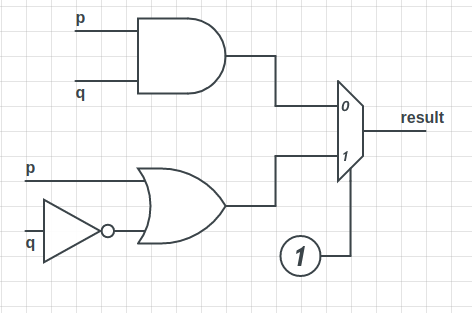
\includegraphics[scale=0.5]{circuit.png}
	\caption{Combinational Circuit}
	\label{fig: circuit}
	
\end{figure*}

\begin{itemize}
    \item p : It is sunny.
    \item q : The flowers are blooming.
\end{itemize}    


\begin{table4}[]
\begin{tabular}{|l|l|l|l|l|}
\hline
p & q & \begin{tabular}[c]{@{}l@{}}$ \rightharpoondown$q\end{tabular} & p $\wedge$ q & \begin{tabular}[c]{@{}l@{}}p \vee $ \rightharpoondown$ q\end{tabular} \\ \hline
T & T & F                                                               & T         & T                                                                      \\ \hline
T & F & T                                                               & F         & T                                                                      \\ \hline
F & T & F                                                               & F         & F                                                                      \\ \hline
F & F & T                                                               & F         & T                                                                      \\ \hline
\end{tabular}
\end{table4}

\newline\newline\newline

\begin{itemize}
    
\end{itemize}

    Circuit can be expressed as (p $\wedge$ q ) Multiplexer  (p $\vee$ $\rightharpoondown$ q ) \newline
    Multiplexer selection is 1\newline
    These 3 are connected to OR gate\newline
    Circuit becomes \newline
    
    Multiplexer is 1 so result will be p $\vee$ $\rightharpoondown$ q \newline
    It means It is sunny or The flowers are not blooming
    \newline
    \newline

\begin{figure*}[htp]
	\centering
	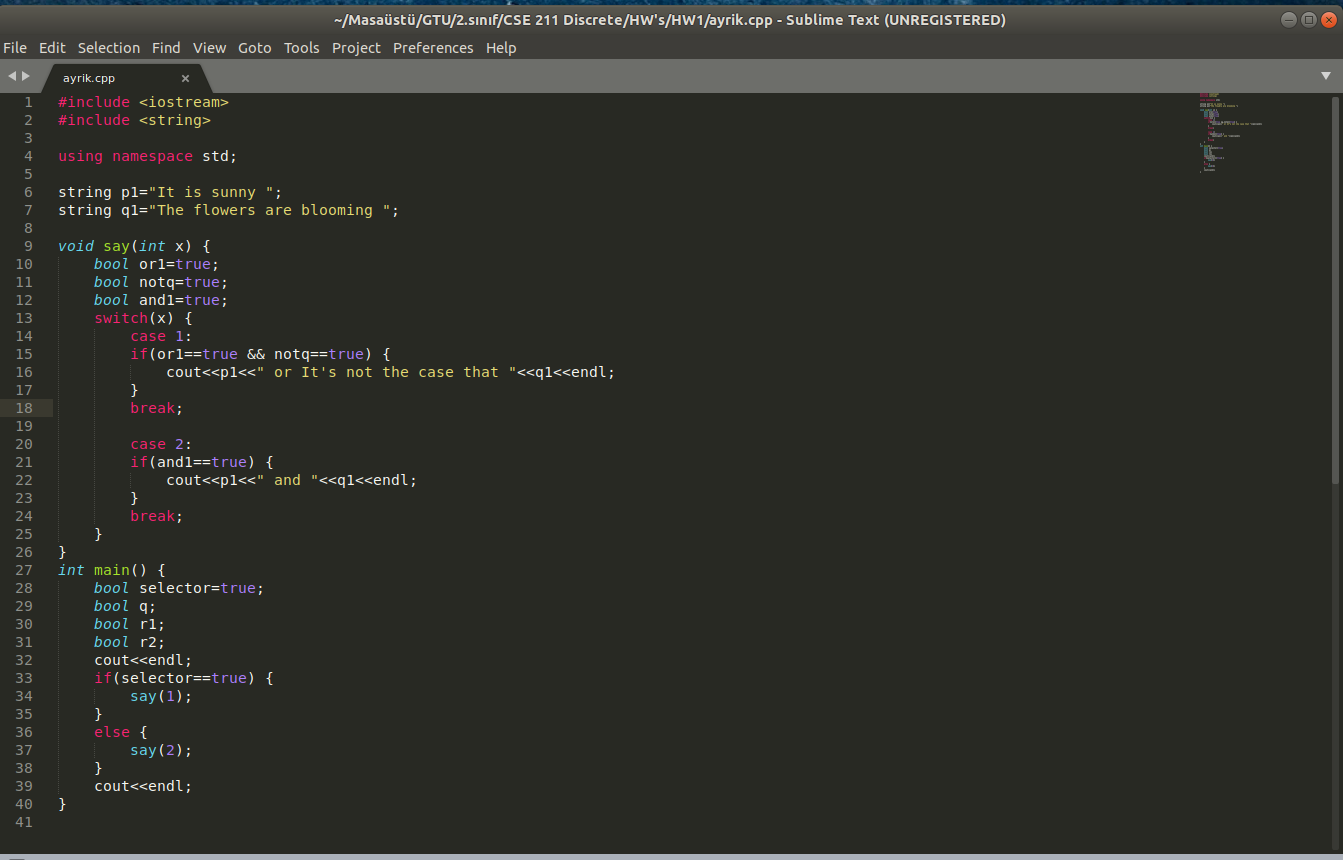
\includegraphics[scale=0.5]{code.png}
	\caption{Code}
	\label{fig: circuit}
	
\end{figure*}





   
   
    



   


\end{document}

